\documentclass[tikz,border=5pt]{standalone}
\usetikzlibrary{calc}
\begin{document}
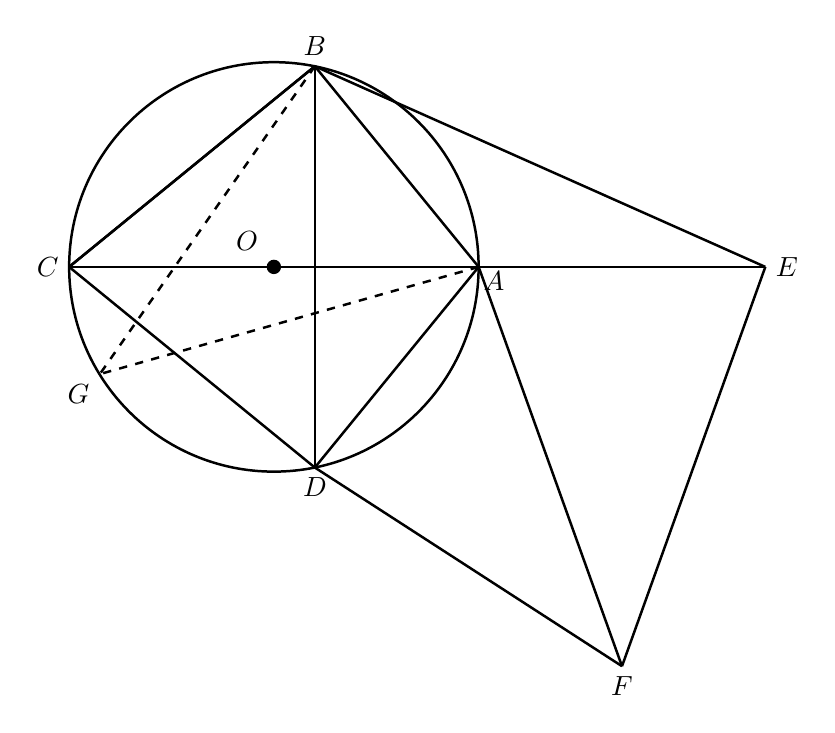
\begin{tikzpicture}[scale=1.3,line width=0.9pt]
  % circle and center
  \coordinate (O) at (0,0);
  \coordinate (C) at (-2,0);
  \coordinate (A) at (2,0);
  \coordinate (B) at (0.4,1.9596);
  \coordinate (D) at (0.4,-1.9596);
  \coordinate (G) at (-1.7,-1.0471);
  \coordinate (E) at (4.8,0);
  \coordinate (F) at (3.4,-3.9);

  \draw (O) circle (2);
  \fill (O) circle (2pt) node[above left=2pt] {$O$};

  % horizontal line: C - O - A - E all solid
  \draw (C) -- (E);
  % note: AO is drawn as part of C--E; redraw AO dashed on top? 
  % Instead draw segments explicitly:
  \draw (C) -- (O);          % OC solid
  \draw[dashed] (O) -- (A);  % AO dashed (edit)
  \draw (A) -- (E);          % EA solid

  % cyclic quadrilateral + diagonals
  \draw (C) -- (B);
  \draw (B) -- (A);
  \draw (C) -- (D);
  \draw (B) -- (D);
  \draw (A) -- (D);
  \draw (B) -- (C);

  % dashed lines to G
  \draw[dashed] (B) -- (G);
  \draw[dashed] (A) -- (G);

  % outer construction
  \draw (B) -- (E);
  \draw (E) -- (F);
  \draw (A) -- (F);
  \draw (D) -- (F);

  % labels
  \node[left] at (C) {$C$};
  \node[above] at (B) {$B$};
  \node[below right=-2pt] at (A) {$A$};
  \node[below] at (D) {$D$};
  \node[below left] at (G) {$G$};
  \node[right] at (E) {$E$};
  \node[below] at (F) {$F$};
\end{tikzpicture}
\end{document}
